\documentclass[11pt, a4paper]{article}

%\usepackage[T1]{fontenc}
%\usepackage{fullpage}

\usepackage[utf8]{inputenc} % comment when using lualatex
\usepackage[italian]{babel} % lingua e a-capo-sillabato
\usepackage{graphicx}
\usepackage[hidelinks]{hyperref} % link di pagina
\usepackage[bottom]{footmisc} % note appiccicate al fondo della pagina
\usepackage{float} % per posizionamento immagini
\usepackage{amsthm} % per ambienti stile teorema
\usepackage{tabularx} %tabelle
\usepackage[table]{xcolor} %colore caselle
\usepackage{enumitem} %additional commands for lists
\usepackage{fancyhdr}



\pagestyle{fancy}
\fancyhf{}% Clear header/footer
\fancyhead[C]{\footnotesize\textit{Documento:} D2 \hfill SleepCode \hfill \textit{Versione:} 1.0}
\renewcommand{\headrule}{{\color{red!70}\rule{\textwidth}{2pt}}}
\setlength{\headheight}{22pt}

\renewcommand\UrlFont{\color{blue}\rmfamily} % colore link

\theoremstyle{definition} % stile dei newtheorem (non italizzati)
\newtheorem{funcreq}{RF} %% numerazione dei requisiti funzionali
\newtheorem{nonfuncreq}{RNF} %% requisiti non funzionali
\newtheorem{backend}{BE}
\newtheorem{frontend}{FE}




\title{Specifica dei Requisiti}

\author{Raffaele \textsc{Castagna}\\
Alberto \textsc{Rovesti}\\
Zeno \textsc{Saletti}}

\newcommand{\groupNumber}{G17}

% Web address for the project (if any)
% \newcommand{\homepage}{\url{https://www.}}

% data
\date{\today}

\makeatletter{}

% IL PREAMBOLO FINISCE QUI %%%%%%%%%%%%%%%%%%%%%%%%%%%%%%%%%%%%%%%%%%%%%%%%%%%%



\begin{document}

% La pagina di copertina si trova in un file .tex a parte
% NON MODIFICARE QUESTO COMANDO!!!
\begin{titlepage}
\newcommand{\HRule}{\rule{\linewidth}{0.3mm}} % Defines a new command for horizontal lines, change thickness here
\center % Centre everything on the page

%------------------------------------------------
%	Logo
%------------------------------------------------

\includegraphics[width=0.3\textwidth]{materiale/UniTrento_logo_ITA_colore.png}\\[0.5cm]
%------------------------------------------------
%	Headings
%------------------------------------------------
\textsc{\Large Dipartimento di Ingegneria\\e Scienza dell'Informazione}\\[1.5cm]

{\Huge\textbf{Sleep Code}}\\[0.5cm]
\textsc{\large Progetto per il Corso di Ingegneria del Software}\\
\textsc{\large Anno Accademico 2023-2024}\\[0.5cm]

%------------------------------------------------
%	Title
%------------------------------------------------

\HRule\\[0.4cm]
{\huge\bfseries \@title}\\[0.1cm]
\HRule\\[1cm]

\begin{minipage}{\textwidth}
\begin{flushleft}
\textit{Descrizione:} documento di analisi dei requisiti funzionali, non funzionali, front-end e back-end.
\end{flushleft}
\end{minipage}\\[1.5cm]


\begin{minipage}{0.4\textwidth}
\begin{flushleft}
\large
\textit{Numero documento:} D1
\end{flushleft}
\end{minipage}
\begin{minipage}{0.4\textwidth}
\begin{flushright}
\large
\textit{Versione documento:} 2.4
\end{flushright}
\end{minipage}\\[1.5cm]

%------------------------------------------------
%	Author(s)
%------------------------------------------------
\begin{minipage}{0.4\textwidth}
\begin{flushleft}
\large
\textit{Membri del gruppo:}\\
\@author % Your name
\end{flushleft}
\end{minipage}
~
\begin{minipage}{0.4\textwidth}
\begin{flushright}
\large
\textit{Numero gruppo: }
\groupNumber
\end{flushright}
\end{minipage}

% 	If you don't want a supervisor, uncomment the two lines below and comment the code above
% 	{\large\textit{Author(s)}}\\
% 	\@author % Your name

%------------------------------------------------
%	Date
%------------------------------------------------

\vfill\vfill
\textit{Ultima revisione:}
{\@date}

\end{titlepage}

\tableofcontents

\newpage

\section*{Scopo del documento}
Il presente documento riporta la specifica dei requisiti di sistema
del progetto SleepCode ricorrendo a diagrammi realizzati secono lo
Unified Modeling Language (UML) e tabelle.

\section{Requisiti funzionali}
In questa sezione vengono descritti i requisiti funzionali (RF) del
servizio utilizzando alcuni Use Case Diagrams (UCD) disegnati secondo
gli standard UML, eventualmente arricchiti da descrizioni in linguaggio
naturale.


\subsection{Accesso}
\begin{itemize}
    \item \textbf{RF 1.} Registrazione
    \item \textbf{RF 2.} Login
    \item \textbf{RF 3.} Recupero password
\end{itemize}

\begin{figure}[H]
\centering
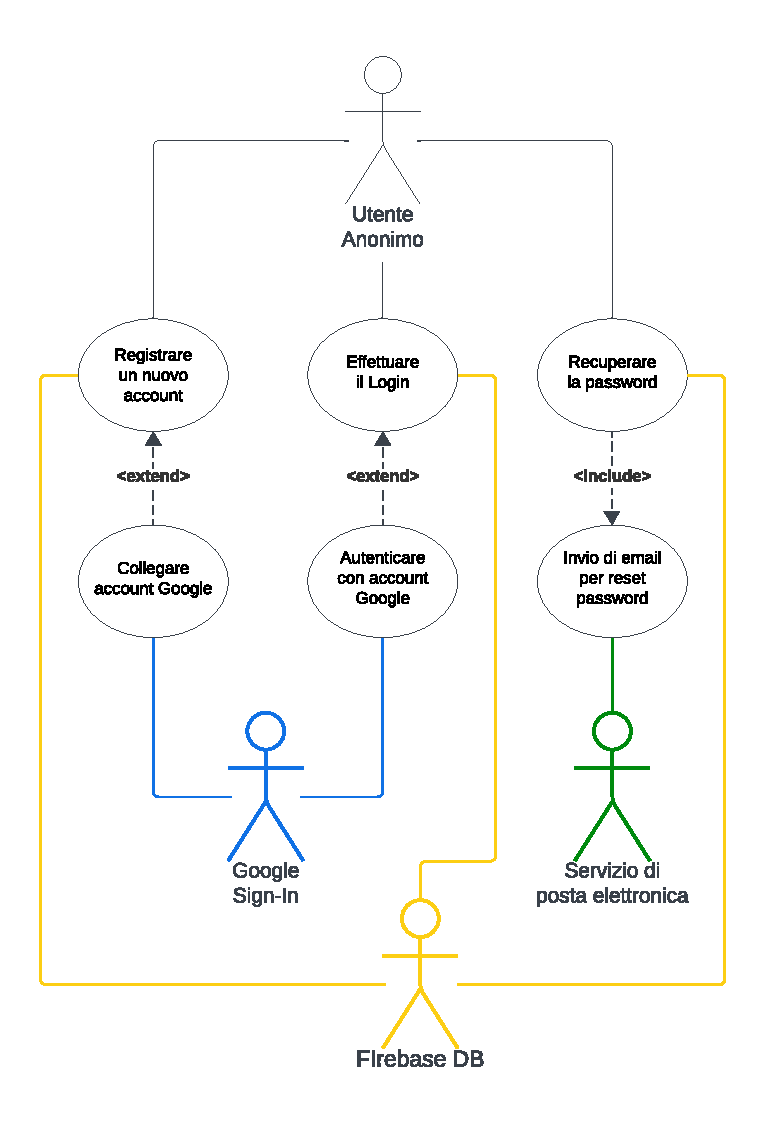
\includegraphics[scale=0.65]{materiale/ucdiagrams/ucaccesso.pdf}
\caption{UCD dello scenario di accesso al servizio}
\end{figure}

\hrule
\subsubsection*{Descrizione Use Case \textit{Registrare un nuovo account}}
\begin{description}
    \item[Titolo:] Registrazione account
    
    \item[Riassunto:] Questo Use Case descrive come l'utente anonimo deve
    effettuare la registrazione sulla piattaforma.

    \item[Descrizione:]
    \begin{enumerate}
        \item[]
        \item L'utente anonimo accede alla pagina dedicata e sceglie tra la registrazione mediante il sistema di credenziali interno oppure per mezzo di un account Google.
        \item La registrazione con sistema di credenziali interno prevede l'inserimento di un username, un'email valida e una password conforme (RNF). \verb|[exception 1]|\verb|[exception 2]|\verb|[exception 3]|
        \item La password deve essere confermata reinserendola in un secondo campo.
        \item L'account viene registrato dal servizio di database.
    \end{enumerate}
    
    \item[Exceptions:]
    \begin{itemize}
        \item[]
        \item \verb|[exception 1]| Se l'email inserita è malformata, inesistente o associata ad un account già registrato, la registrazione non può proseguire e l'utente viene avvisato.
        \item \verb|[exception 2]| Se la password non è conforme, la registrazione non può proseguire e l'utente viene avvisato.
        \item \verb|[exception 3]| Se i campi di inserimento e di conferma della password contengono stringhe che non coincidono, la registrazione non può proseguire e l'utente viene avvisato.
    \end{itemize}
\end{description}

\subsubsection*{Descrizione Use Case \textit{Recuperare la password}}
\begin{description}
    \item[Titolo:] Recupero password
    
    \item[Riassunto:] Questo Use Case descrive come l'utente anonimo e
    registrato alla piattaforma, facendo affidamento al sistema di credenziali
    interno, può recuperare il proprio account qualora la password venisse dimenticata.

    \item[Descrizione:]
    \begin{enumerate}
        \item[]
        \item L'utente accede alla pagina di recupero, per mezzo di quella di login.
        \item La pagina indica all'utente di inserire l'email di recupero, ovvero quella associata all'account. \verb|[exception 1]|
        \item Il sistema richiede al servizio di posta elettronica l'invio di un link di recupero mediane un messaggio email, specificando l'indirizzo fornito dall'utente.
        \item Il link guida l'utente dal messaggio alla pagina del sistema dedicata alla creazione di una nuova password.
        \item L'utente inserisce una nuova password conforme e la conferma, inserendola nuovamente. \verb|[exception 2]|\verb|[exception 3]|
        \item Il servizio di database provvede all'aggiornamento della password.
    \end{enumerate}
    
    \item[Exceptions:]
    \begin{itemize}
        \item[]
        \item \verb|[exception 1]| Se l'email inserita è malformata, inesistente o associata ad un account non registrato, il recupero non può proseguire e l'utente viene avvisato.
        \item \verb|[exception 2]| Se la password non è conforme, la registrazione non può proseguire e l'utente viene avvisato.
        \item \verb|[exception 3]| Se i campi di inserimento e di conferma della password contengono stringhe che non coincidono, la registrazione non può proseguire e l'utente viene avvisato.
    \end{itemize}
    
    %\item[Extensions:]
\end{description}


\newpage
\subsection{Consultazione dei problemi}
\begin{itemize}
    \item \textbf{RF 4.} Consultazione del catalogo dei problemi
    \item \textbf{RF 5.} Consultazione di un problema
    \item \textbf{RF 8.} Metadati aggiuntivi
    \item \textbf{RF 9.1.} Progressi
\end{itemize}
\subsection*{2.5\texttt{ }\textit{ } Gestione del catalogo dei problemi}
\begin{itemize}
    \item \textbf{RF 12.} Aggiungere un problema
    \item \textbf{RF 13.} Modificare un problema
    \item \textbf{RF 14.} Eliminare un problema
\end{itemize}

\begin{figure}[H]
\centering
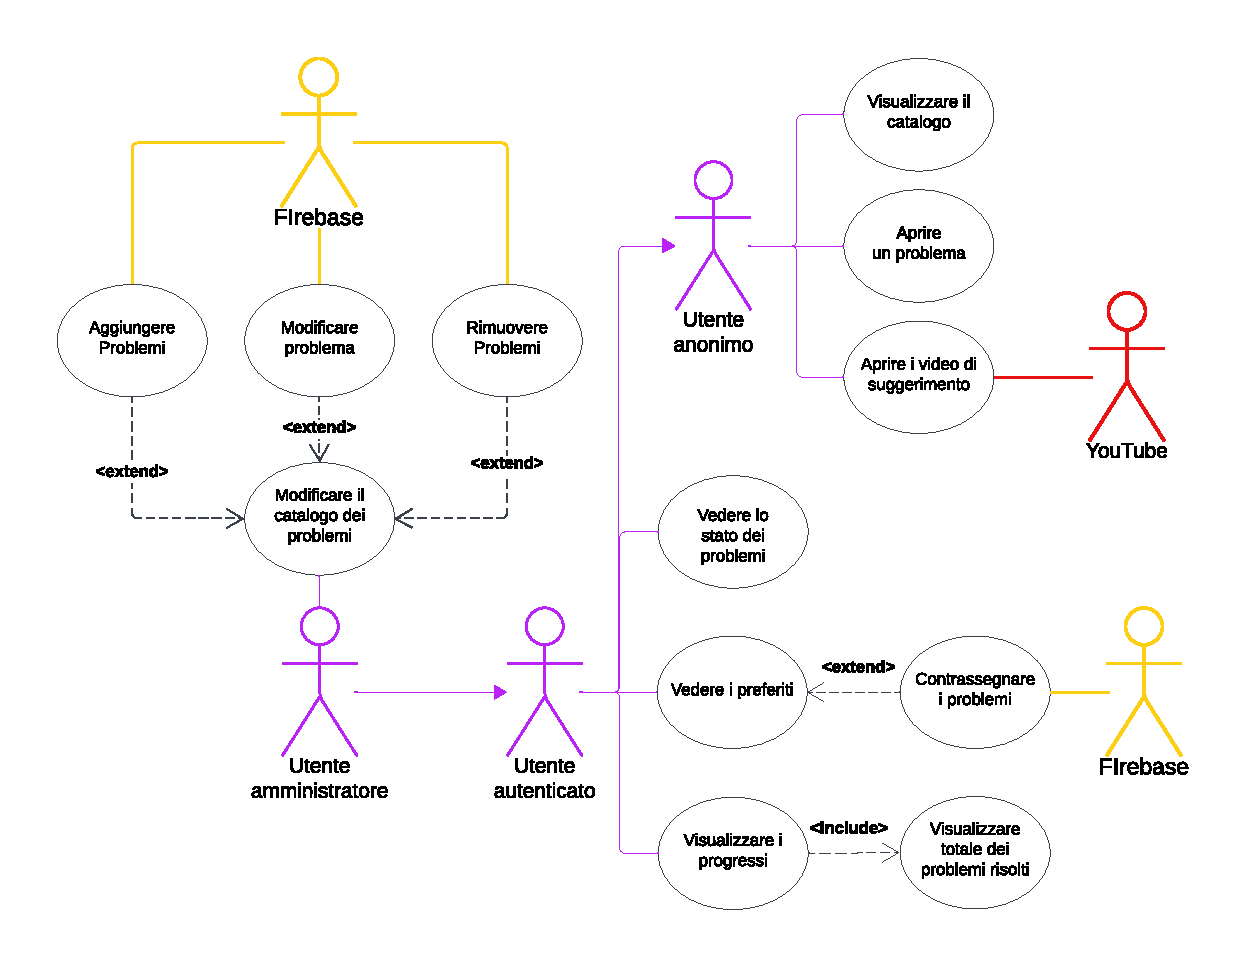
\includegraphics[scale=0.55]{materiale/ucdiagrams/ucproblemi.pdf}
\caption{UCD dello scenario della consultazione dei problemi e della modifica del catalogo}
\end{figure}
\hrule

\subsubsection*{Descrizione Use Case \textit{Aggiungere problemi}}
\begin{description}
    \item[Titolo:] Aggiungere un problema
    
    \item[Riassunto:] Questo Use Case descrive come l'utente amministratore
    deve aggiungere nuovi problemi al catalogo.

    \item[Descrizione:]
    \begin{enumerate}
        \item[]
        \item L'utente amministratore accede alla pagina del catalogo e sceglie di aggiungere un nuovo problema.
        \item L'utente compila i campi necessari alla creazione di un nuovo problema: i dati relativi alla struttura, quali titolo, descrizione e almeno tre esempi di input e output atteso; dati descrittivi, ovvero nome, selezione della difficoltà (bassa, intermedia, alta), categoria e link al video-suggerimento.
        \item L'utente inserisce almeno 3 test cases; ogni test case consiste in un dato in input e il rispettivo output corretto.
        \item L'utente conferma la creazione del problema, che viene quindi aggiunto al catalogo; alternativamente, l'utente può scegliere di annullare la creazione del nuovo problema, previo avviso e conferma da parte del sistema.\texttt{[exception 1]}\texttt{[exception 2]}
    \end{enumerate}
    
    \item[Exceptions:]
    \begin{itemize}
        \item[]
        \item \texttt{[exception 1]} Se tra i dati strutturali e descrittivi del problema è presente almeno un campo non compilato, l'aggiunta del problema al catalogo non viene eseguita e l'utente viene avvisato.
        \item \texttt{[exception 2]} Se il numero di test cases forniti è minore di 3, il problema non può essere aggiunto e l'utente viene notificato.
    \end{itemize}
\end{description}

\subsubsection*{Descrizione Use Case \textit{Modificare problemi}}
\begin{description}
    \item[Titolo:] Modificare un problema
    
    \item[Riassunto:] Questo Use Case descrive come l'utente amministratore
    deve modificare i problemi.

    \item[Descrizione:]
    \begin{enumerate}
        \item[]
        \item L'utente amministratore accede alla pagina del catalogo e seleziona un problema da modificare.
        \item L'utente modifica i campi strutturali (titolo, descrizione, esempi di input e output) e descrittivi (nome, difficoltà, categoria e link al video-suggerimento) del problema.
        \item L'utente modifica i test cases, aggiungendone eventualmente più di 3.
        \item L'utente conferma la modifica del problema, che verrà poi aggiornato nel catalogo, oppure conferma di annullare la modifica.\texttt{[exception 1]} \texttt{[exception 2]}
    \end{enumerate}
    
    \item[Exceptions:]
    \begin{itemize}
        \item[]
        \item \texttt{[exception 1]} Se tra i dati strutturali e descrittivi del problema è presente almeno un campo non compilato, la modifica del problema non viene eseguita e l'utente viene avvisato.
        \item \texttt{[exception 2]} Se il numero di test cases forniti è minore di 3, il problema non può essere modificato e l'utente viene notificato.
    \end{itemize}

    \item[Extensions:]
    \begin{itemize}
        \item[]
        \item \verb|[extension 1]|
    \end{itemize}
\end{description}

\newpage
\subsection{Esercitazione}
\begin{itemize}
    \item \textbf{RF 6.} Avviare l'esercitazione
    \item \textbf{RF 7.} Correttezza dell'algoritmo
    \item \textbf{RF 9.1.} Registrare i progressi
\end{itemize}

\begin{figure}[H]
\centering
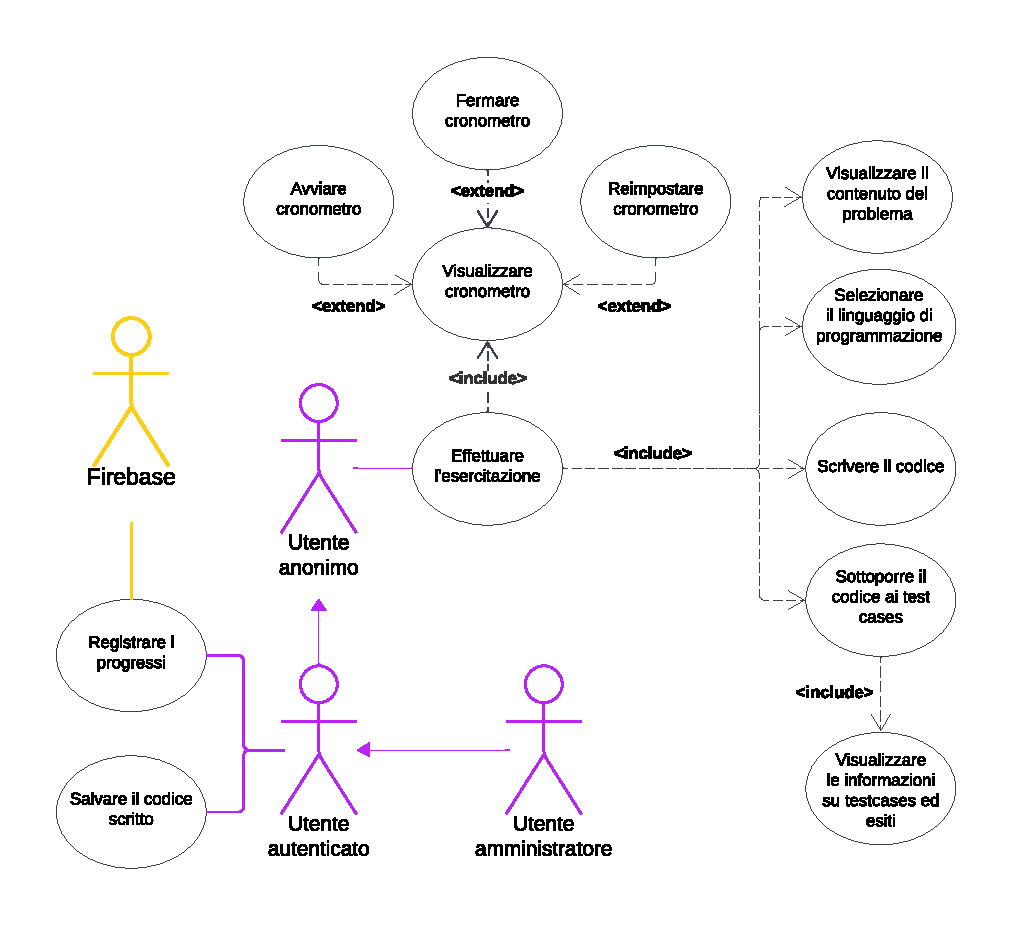
\includegraphics[scale=0.57]{materiale/ucdiagrams/ucesercitazione.pdf}
\end{figure}

\subsubsection*{Descrizione Use Case \textit{Effettuare l'esercitazione}}
% qualche diagrammino più appropriato sarebbe bello

\subsubsection*{Descrizione Use Case \textit{Registrare i progressi}}

\newpage
\subsection{Gestione del profilo e dell'account}
\begin{itemize}
    \item \textbf{RF 9.2.} Progressi
    \item \textbf{RF 10.} Aggiornamento dei dati dell'account
    \item \textbf{RF 11.} Logout
\end{itemize}

\begin{figure}[H]
\centering
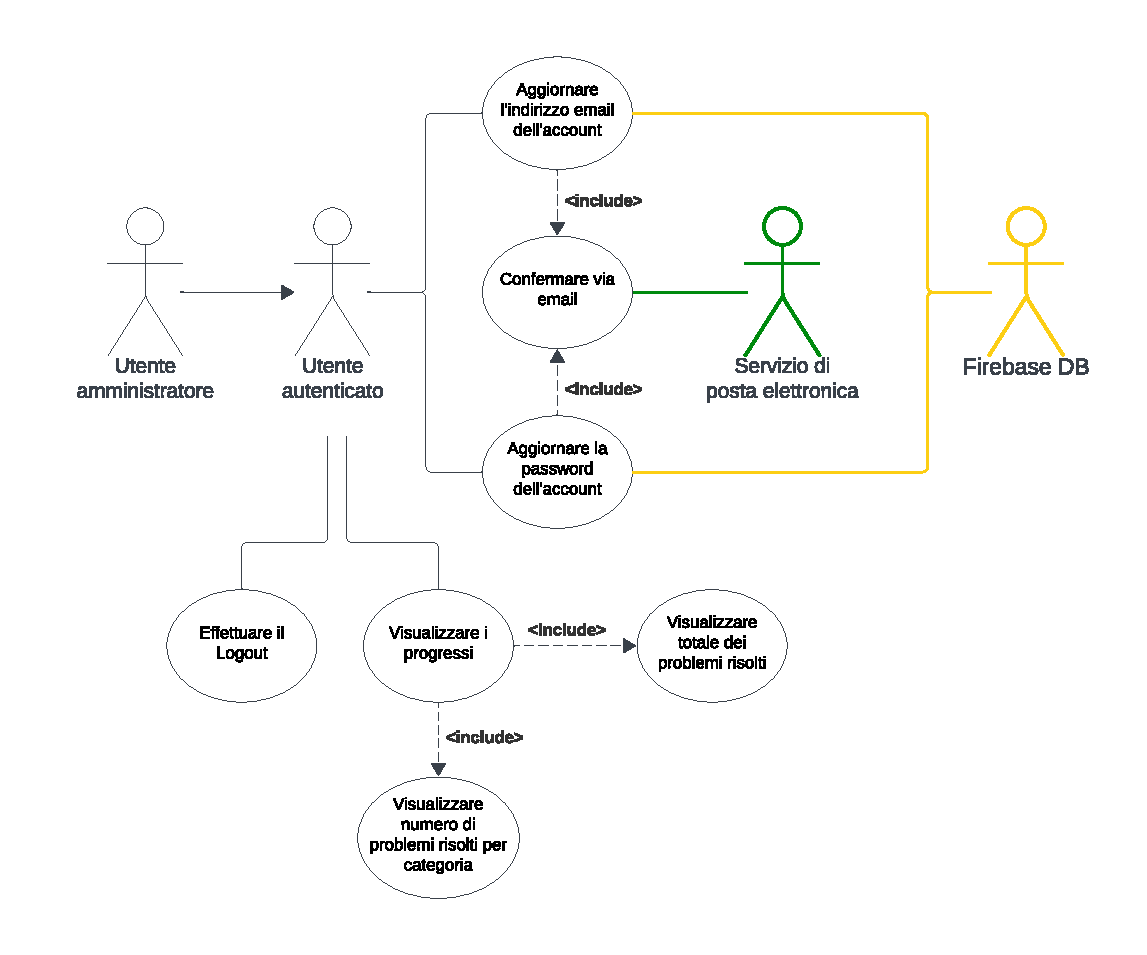
\includegraphics[scale=0.8]{materiale/ucdiagrams/ucaccount.pdf}
\caption{UCD dello scenario con le funzionalità aggiuntive dell'utente autenticato}
\end{figure}
\hrule

\subsubsection*{Descrizione Use Case \textit{Aggiornare l'indirizzo email dell'account}}
\subsubsection*{Descrizione Use Case \textit{Aggiornare la password dell'account}}



\newpage
\section{Requisiti non funzionali}
Nella presente sezione sono riportati i requisiti non funzionali (RNF)
del sistema utilizzando tabelle strutturate. Per ogni requisito vengono
specificat

\subsection{Caratteristiche di sistema}

\begin{nonfuncreq}
\textbf{Scalabilità }
\begin{center}
    \footnotesize
    \begin{tabularx}{\textwidth}{|X||X||X|}
        \hline
        \cellcolor{red!70}Proprietà & \cellcolor{red!70}Descrizione & \cellcolor{red!70}Misura\\
        \hline
        Elaborazione con un numero crescente di utenti. & Capacità del sistema di gestire un numero crescente di utenti in simultanea. & Viene garantito l'accesso in simultanea di almeno 300 utenti nel primo anno dal lancio.\\
        \hline
        Memorizzazione dei dati degli utenti & Capacità del sistema di gestire i dati generati da un numero crescente di utenti utilizzatori. & Capacità sufficiente per almeno 400 utenti.\\
        \hline
        Linguaggi di programmazione & Capacità di supportare un numero crescente di linguaggi di programmazione, utili alla scrittura degli algoritmi risolutivi. & Al lancio della piattaforma, vengono supportate le versioni maggiormente utilizzate dei linguaggi di programmazione più popolari (C++11). Il sistema può gestire algoritmi scritti in almeno 5 linguaggi differenti.\\
        \hline
    \end{tabularx}
\end{center}
\end{nonfuncreq}

\begin{nonfuncreq}
    \textbf{Compatibilità }
    \begin{center}
        \footnotesize
        \begin{tabularx}{\textwidth}{|X||X||X|}
            \hline
            \cellcolor{red!70}Proprietà & \cellcolor{red!70}Descrizione & \cellcolor{red!70}Misura\\
            \hline
            Compatibilità client & La piattaforma del servizio deve essere compatibile con e accessibile attraverso le versioni più recenti dei principali browser in commercio. &
            \begin{itemize}
                \item Chrome

                117.0.5938.150
                \item Firefox

                18.0.1
                \item Edge:

                17.0.2045.60
            \end{itemize}La compatibilità deve valere anche per le rispettive versioni superiori.\\
            \hline
        \end{tabularx}
    \end{center}
\end{nonfuncreq}

\begin{nonfuncreq}
    \textbf{Usabilità }
    \begin{center}
        \footnotesize
        \begin{tabularx}{\textwidth}{|X||X||X|}
            \hline
            \cellcolor{red!70}Proprietà & \cellcolor{red!70}Descrizione & \cellcolor{red!70}Misura\\
            \hline
            Usabilità & Intuitività e facilità nell'apprendimento, accesso e impiego delle funzionalità fornite dal servizio. & Il nuovo utente deve poter conoscere e utilizzare il 90\% delle funzionalità (disponibili al proprio livello di accesso) in meno di 30 minuti.\\
            \hline
        \end{tabularx}
    \end{center}
\end{nonfuncreq}

\begin{nonfuncreq}
    \textbf{Aspetto }
    \begin{center}
        \footnotesize
        \begin{tabularx}{\textwidth}{|X||X||X|}
            \hline
            \cellcolor{red!70}Proprietà & \cellcolor{red!70}Descrizione & \cellcolor{red!70}Misura\\
            \hline
            Colore & Gamma cromatica dell'interfaccia e distribuzione del colore. La scelta ricade su colori, tinte (aggiunta di bianco) e sfumature (aggiunta di nero) che mirano a limitare l'affaticamento della vista. & Colori caldi; colori freddi presenti in sfumature scure; colori freddi accesi presenti al più in aree ristrette (pulsanti e icone).\\
            \hline
            Contrasto & Accostamento dei colori all'interno dell'interfaccia utente. Mira alla leggibilità e alla limitazione dell'affaticamento della vista. & Regola dei complementari; cerchio di Itten.\\
            \hline
        \end{tabularx}
    \end{center}
\end{nonfuncreq}

\begin{nonfuncreq}
    \textbf{Lingua }
    \begin{center}
        \footnotesize
        \begin{tabularx}{\textwidth}{|X||X||X|}
            \hline
            \cellcolor{red!70}Proprietà & \cellcolor{red!70}Descrizione & \cellcolor{red!70}Misura\\
            \hline
            Lingua di sistema           & Lingua presente nell'interfaccia e nelle risorse fornite dal servizio. & L'interfaccia generale della piattaforma contiene testo in italiano (100\%); i testi dei problemi sono scritti in italiano (100\%); le risorse multimediali (video-suggerimento) devono essere in italiano oppure in inglese.\\
            \hline
        \end{tabularx}
    \end{center}
\end{nonfuncreq}

\begin{nonfuncreq}
    \textbf{Prestazioni }
    \begin{center}
        \footnotesize
        \begin{tabularx}{\textwidth}{|X||X||X|}
            \hline
            \cellcolor{red!70}Proprietà & \cellcolor{red!70}Descrizione & \cellcolor{red!70}Misura\\
            \hline
            Caricamento all'accesso & Tempo massimo richiesto per caricare le pagine rilevanti dopo la ricerca in browser. & Il caricamento delle pagine di login e home (per quest'ultima si considera l'intervallo di tempo che comincia dopo la richiesta di autenticazione) non deve eccedere i 2 secondi.\\
            \hline
            Transizioni & Tempo massimo richiesto per effettuare una transizione da una pagina all'altra.  & Una transizione non deve richiedere più di 2 secondi.\\
            \hline
        \end{tabularx}
    \end{center}
\end{nonfuncreq}

\subsection{Affidabilità}

\begin{nonfuncreq}
    \textbf{Downtime }
    \begin{center}
        \footnotesize
        \begin{tabularx}{\textwidth}{|X||X||X|}
            \hline
            \cellcolor{red!70}Proprietà & \cellcolor{red!70}Descrizione & \cellcolor{red!70}Misura\\
            \hline
            Downtime & Tempo medio massimo in cui il servizio non è raggiungibile; principalmente per motivi di manutenzione e aggiornamento. & 2,7\% (240 ore) nel primo anno 0,85\% (72 ore) dopo il primo anno dal lancio.\\
            \hline
        \end{tabularx}
    \end{center}
\end{nonfuncreq}

\begin{nonfuncreq}
    \textbf{Disponibilità }
    \begin{center}
        \footnotesize
        \begin{tabularx}{\textwidth}{|X||X||X|}
            \hline
            \cellcolor{red!70}Proprietà & \cellcolor{red!70}Descrizione & \cellcolor{red!70}Misura\\
            \hline
            Disponibilità & Probabilità che il sito non si guasti entro un intervallo di tempo trascorso dopo l'entrata in servizio. & Probabilità di resistere ai guasti al 98\% entro le prime 8.000 ore.\\
            \hline
        \end{tabularx}
    \end{center}
\end{nonfuncreq}

\subsection{Privacy e sicurezza}

\begin{nonfuncreq}
    \textbf{Privacy e trattamento dei dati }
    \begin{center}
        \footnotesize
        \begin{tabularx}{\textwidth}{|X||X||X|}
            \hline
            \cellcolor{red!70}Proprietà & \cellcolor{red!70}Descrizione & \cellcolor{red!70}Misura\\
            \hline
            Normativa & Conformità con le vigenti norme relative al trattamento e alla protezione dei dati (GDPR). In particolare, i dati personali dell'utente registrato (nome, email e password) non devono essere divulgati in alcun modo e, qualora lo ritenga opportuno, l'utente ha il diritto di richiedere l'eliminazione delle proprie informazioni dal servizio al fine di interrompere il trattamento. & Conformità del servizio e funzionalità a supporto dell'utente (eliminazione account).\\
            \hline
        \end{tabularx}
    \end{center}
\end{nonfuncreq}

\begin{nonfuncreq}
    \textbf{Connessione sicura }
    \begin{center}
        \footnotesize
        \begin{tabularx}{\textwidth}{|X||X||X|}
            \hline
            \cellcolor{red!70}Proprietà & \cellcolor{red!70}Descrizione & \cellcolor{red!70}Misura\\
            \hline
            Connessione sicura & Impiego di protocolli di comunicazione che garantiscono la confidenzialità e riservatezza delle informazioni scambiate tra client e server. & Utilizzo del protocollo \texttt{https}.\\
            \hline
        \end{tabularx}
    \end{center}
\end{nonfuncreq}

\begin{nonfuncreq}
    \textbf{Password strength }
    \begin{center}
        \footnotesize
        \begin{tabularx}{\textwidth}{|X||X||X|}
            \hline
            \cellcolor{red!70}Proprietà & \cellcolor{red!70}Descrizione & \cellcolor{red!70}Misura\\
            \hline
            Password sicura & Quantità e varietà di caratteri necessari per comporre una password forte. & Una password conforme possiede da 8 a 64 caratteri, tra i quali sono presenti almeno: una lettera maiuscola, una minuscola, una cifra decimale e un carattere speciale tra ! ? \# \$ \% \& @ * + - / $\backslash$ = \_ . , ; : ( ) [ ] \{ \}.\\
            \hline
        \end{tabularx}
    \end{center}
\end{nonfuncreq}





\newpage
\section{Analisi del contesto}
% riguarda il backend e i componenti esterni al sistema: tutto il codice che utilizzate ma che non avete scritto voi
% flusso di informazioni tra il nostro sistema e quelli esterni
In questa sezione viene descritto il contesto di funzionamento del sistema
\textit{SleepCode} e come esso interagisce con gli attori esterni. Si
ricorre ad una descrizione testuale riassunta in una rappresentazione
grafica mediante un Diagramma di Contesto (Figura \ref{contextdiagram}).

\subsection{Utenti e sistemi esterni} % chi interagisce, chi usa e chi supporta (sia software che umano)
\subsubsection{Utente}
L'utente rappresenta l'attore che usufruisce delle funzionalità del servizio
—viene descritto nei requisiti dal \textbf{RF 1} al \textbf{RF 7} per quanto
concerne il livello anonimo e quelli superiori; dal \textbf{RF 8} al
\textbf{RF 11} in relazione ai livelli autenticato e amministratore; \textbf{RF 12},
\textbf{RF 13} e \textbf{RF 14} per quanto riguarda il livello amministratore.

\subsubsection{Firebase DB}
Il servizio di database impiegato per gestire le credenziali e l'account
degli utenti registrati alla piattaforma—i requisiti coinvolti sono: \textbf{RF 1},
\textbf{RF 2}, \textbf{RF 3}, \textbf{RF 9}, \textbf{RF 10}—e per gestire il
catalogo dei problemi—\textbf{RF 12}, \textbf{RF 13}, \textbf{RF 14}.

\subsubsection{Google Sign-In}
Servizio di autenticazione alternativo al sistema di credenziali interno
—\textbf{RF 1}, \textbf{RF 2}.

\subsubsection{YouTube}
Il servizio di contenuti multimediali che fornisce i video che integrano
i problemi, mettendo a disposizione dell'utente un suggerimento per lo
svolgimento dell'esercizio—\textbf{RF 4.1}, \textbf{RF 6.6}.

\subsubsection{Servizio di posta elettronica}
Sistema di notifica utilizzato per effettuare le operazioni di recupero
dell'account (\textbf{RF 3}) e di migrazione a nuovo indirizzo di posta
elettronica da associare all'account (\textbf{RF 10}).

\subsection{Diagramma di contesto} % frecce = dati che si scambiano. Utente --atuenticaz--> sistema (è l'utente che fornisce i dati al sistema; la freccia indica il verso del flusso)
\begin{figure}[H]
\centering
\hspace*{-1.8cm}
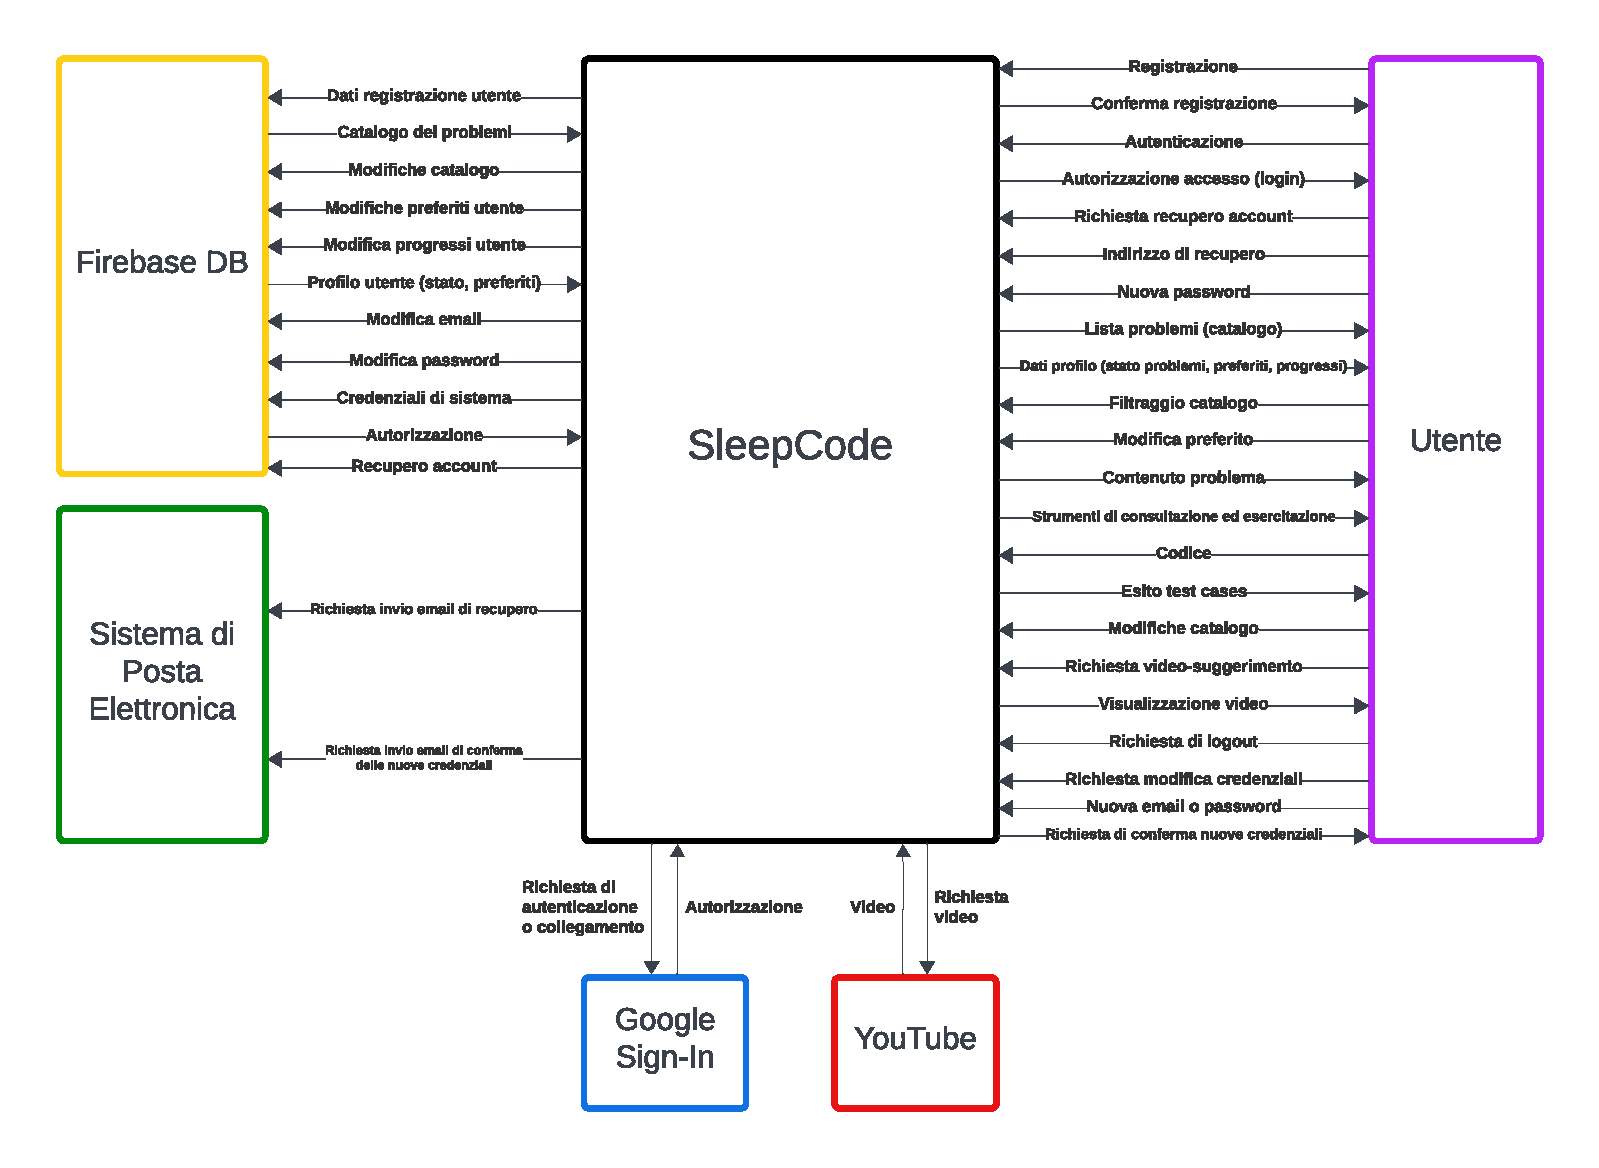
\includegraphics[scale=0.6]{materiale/contextdiagram.pdf}
\caption{Context Diagram della piattaforma \textit{SleepCode}}
\label{contextdiagram}
\end{figure}

L'utente può richiedere di effettuare la registrazione alla piattaforma
(\textbf{RF 1}), scegliendo di inviare i dati necessari per creare un
account di sistema o di collegare il proprio account Google. Il sistema
provvede a inviare la conferma dell'operazione di registrazione.

L'utente registrato può inviare i dati necessari al login (\textbf{RF 2}) sulla piattaforma,
inserendo quindi le credenziali di sistema oppure richiedendo l'autenticazione
con Google. Il sistema risponde con l'autorizzazione all'accesso.

In caso di richiesta di recupero dell'account (\textbf{RF 3}) da parte di un utente
registrato, il sistema riceve l'indirizzo email di recupero. Dall'email
l'utente può collegarsi alla pagina di recupero, nella quale inserire la
nuova password dell'account.
\\\\
I video che l'utente intende visualizzare vengono richiesti a YouTube da
parte del sistema.
\\\\
Google Sign-In fornisce l'autorizzazione al collegamento e all'accesso
mediante account Google, richiesti da utenti in sede di registrazione o
login.
\\\\
La piattaforma fornisce al sistema di posta elettronica i dati necessari
per notificare e guidare l'utente che intende effettuare alcune operazioni,
ovvero la registrazione e la modifica dei dati dell'account.



\newpage
\section{Analisi dei componenti}
% diagramma componenti -> si intende componenti INTERNI AL SISTEMA:

% vantaggi componenti: se cambia uno degli attori (in particolare software)
% basta cambiare il rispettivo compnente con il quale si interfaccia

% il sistema non sarà un programma monolitico che si occupa di tutto con un unico codice
% provo a dividere il mio sistema in componenti e ragiono su come le informazioni vengono passate tra i componenti

Nella sezione seguente viene descritta l'architettura interna del sistema
rilevandone i componenti, definiti nei loro compiti sulla base dei requisiti
analizzati nelle sezioni e nei documenti precedenti. L'architettura viene
qui mostrata attraverso un Diagramma dei Componenti, che evidenzia
l'interconnessione tra i componenti interni, le interfacce presenti tra di
essi e quelle esposte agli attori esterni. Segue una descrizione testuale
e più dettagliata di ogni componente.


\subsection{Definizione dei componenti}
\subsection{Diagramma dei componenti}

\end{document}